\documentclass[12pt]{article}

\usepackage{url}
\usepackage{fullpage}
\usepackage{graphicx}
\usepackage{amsmath,amssymb}

\newcommand{\eps}{\varepsilon}
\newcommand{\R}{\mathbb{R}}
\newcommand{\inprod}[1]{\langle #1 \rangle}

\DeclareMathOperator*{\E}{\mathbb{E}}
\let\Pr\relax
\DeclareMathOperator*{\Pr}{\mathbb{P}}

\begin{document}

\thispagestyle{empty}

\begin{center}
{\Large \textsc{CS 294-165 Sketching Algorithms} --- Fall 2020}

\bigskip

{\Large \textsc{Problem Set 1}}

\smallskip

Due: 11:59pm, Friday, October 16th

\bigskip

{\footnotesize See homework policy at \url{http://www.sketchingbigdata.org/fall20/syllabus/}}

{\footnotesize Each problem is worth 15 points (except Problem 4).}
\end{center}

\paragraph{Problem 1: Incoherent matrices.} A matrix $\Pi\in\R^{m\times n}$ is {\em $\epsilon$-incoherent} if
\begin{enumerate}
  \item For each column $\Pi^i$,  $\|\Pi^i\|_2 = 1$.
\item For each $i\neq j$, $|\inprod{\Pi^i, \Pi^j}| < \epsilon$.
  \end{enumerate}

  In the lecture notes, Theorem 3.1.4 implies that for any $n> 1$ and $\epsilon\in(0,1)$, there exists a code $\mathcal C$ with $n$ codewords, alphabet size $q=O(1/\epsilon)$, block length $\ell = O(\epsilon^{-1}\log n)$, and relative distance $1-\epsilon$. This leads to an $\epsilon$-incoherent matrix via the construction in Figure~\ref{fig:codes}, where the columns of $\Pi$ are in correspondence with codewords in $\mathcal C$.

  \begin{figure}[!h]
\begin{center}
\scalebox{0.8}{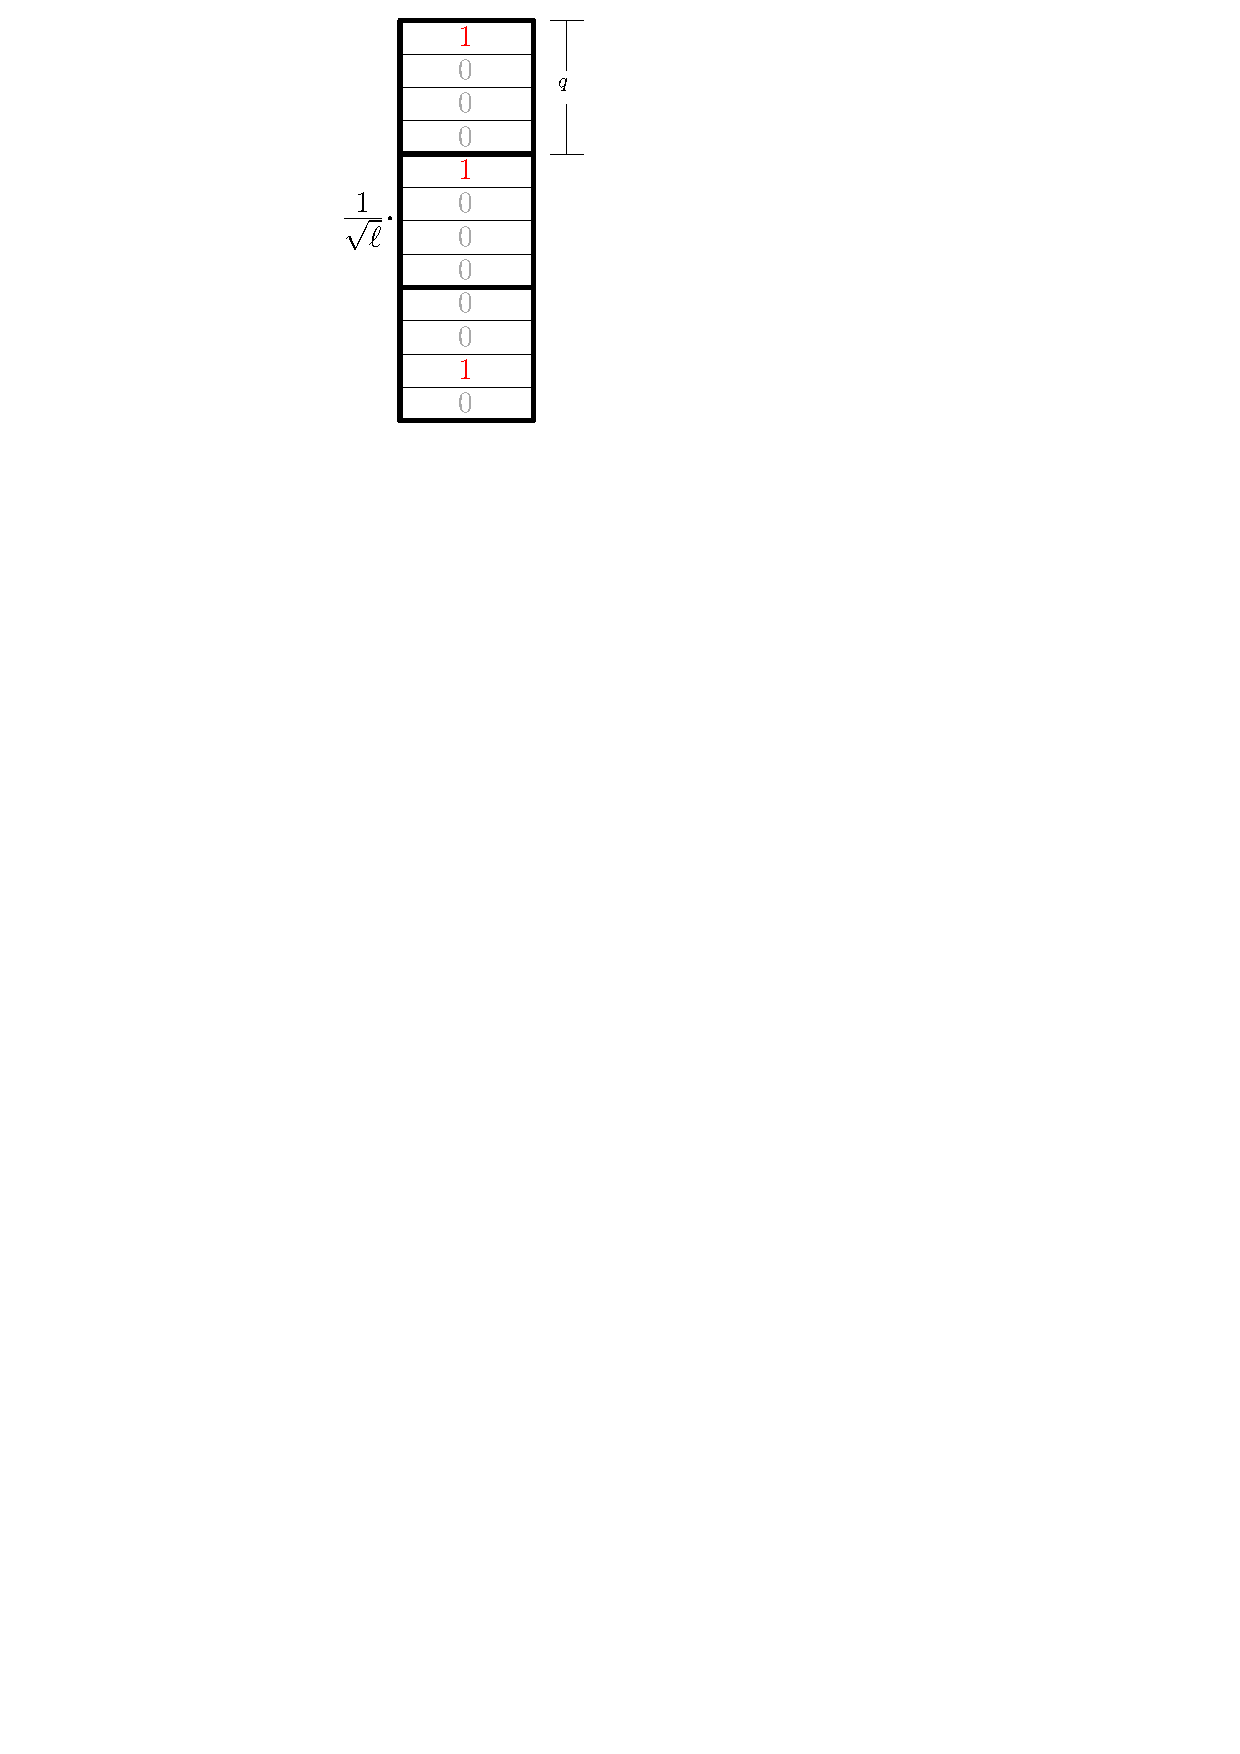
\includegraphics{code_vector}}
\caption{Each codeword gives one column of the incoherent matrix. Here $q = 4, t = 3$ and the codeword is $C_i = (1,1,3)$. The vector is $m = qt$ dimensional with the coordinates broken up into $t$ blocks each of size $q$. A $1$ is placed in the $j$th position in the location specified by $(C_i)_j$. The entire vector is normalized by $1/\sqrt{\ell}$ to have unit norm.}\label{fig:codes}
\end{center}
\end{figure}

\vspace{-.2in}\begin{itemize}
  \item[(a)] (2 points) Consider the construction in Figure~\ref{fig:codes} to convert a code with $n$ codewords, block length $\ell$, alphabet size $q$, and relative distance $\rho$ into a matrix $\Pi\in\R^{m\times n}$. For what $\epsilon$ is it $\epsilon$-incoherent? How many rows $m$ does it have? Your answers should be in terms of the code parameters.
  \end{itemize}

  It turns out one can achieve a better $m$ than the code of Theorem 3.1.4 when $\epsilon$ is sufficiently small. Suppose the alphabet size $q$ is a prime power and consider the finite field $\mathbb{F}_q$. Consider all polynomials $p_1,\ldots,p_N\in \mathbb{F}_q[x]$ of degree at most $d$ where $N = q^{d+1}$. Define the {\em Reed-Solomon code} $C_1,\ldots,C_N$ as follows: $\ell = q$ where the $j$th entry of $C_i$ is the evaluation of $p_i$ on the $j$th element of $\mathbb{F}_q$ (so $C_i$ is the evaluation table of $p_i$).

\begin{itemize} 
\item[(b)] (5 points) If we still want to have at least $n$ codewords, we need $N \ge n$. Show how to choose $d,q$ so $N \ge n$ and the relative distance is $1-\epsilon$, and show what this gives (in big-Oh notation) for the number $m$ of rows of the incoherent matrix $\Pi$ we obtain.
\item[(c)] (3 points) How small does $\epsilon$ need to be as a function of $n$ for the codes from part (b) to give smaller $m$ than the code from Theorem 3.1.4? If the turning point is $\epsilon_T$, you should provide an answer $\epsilon'_T$ such that $\log(1/\epsilon'_T) = \Theta(\log(1/\epsilon_T))$.
\item[(d)] (5 points) Suppose one has an $\epsilon$-incoherent matrix $\Pi$. Show how $\ell_1$-point queries to $x$ being updated in the turnstile streaming model can be answered solely given $y = \Pi x$. (Note then that part (b) implies a {\em deterministic} $\ell_1$-point query algorithm with low space in turnstile streams.) \textbf{Hint:} it may  help to remember that $\Pi x = \sum_i x_i \Pi^i$.
\end{itemize}


\noindent \textbf{OPEN PROBLEM:} It is known that any $\epsilon$-incoherent matrix with $n$ columns must have $m = \Omega(\min\{n, \epsilon^{-2}(\log n)/\log(1/\eps))\}$ \cite[Section 9]{Alon03}. Can the gap between upper and lower bounds be closed? It is conceivable a better upper bound could be achieved by discovering a better code construction.

\paragraph{Problem 2: Counting distinct elements with deletions.}  In Lecture 2 we showed how to estimate the number of distinct elements in a stream in $\mathop{poly}(\eps^{-1}\lg n)$ bits of space with $2/3$ success probability, where all integers in the stream are in $[n]$. In Lecture 3, we gave a different algorithm based on geometric sampling. Recall in the turnstile model, the distinct elements problem asks us to estimate $\|x\|_0 := |\{i : x_i\neq 0\}|$ when all updates have $\Delta=+1$. What if the updates in the stream are allowed to have $\Delta\in\{-1,1\}$ though? Show how to alter the geometric sampling algorithm from Section 2.2.3 of the lecture notes to also handle such negative updates. What is the space complexity of your solution? Any solution using space $\mathop{poly}(\eps^{-1}\lg (nL))$ for this modified problem, where $L$ is the length of the stream, will receive full credit.

\paragraph{Problem 3: Insertion-only $\ell_1$ heavy hitters.}

In class we considered {\em turnstile streams} where a vector $x\in\R^n$ receives updates of the form ``add $\Delta$ to $x_i$'' in a stream. As mentioned, {\em insertion-only streams} are a special case of turnstile streams where $\Delta=1$ always (so we can just imagine the stream is a sequence $i_1 i_2 \cdots i_L$ of integers in $[n]$). Also, recall in the point query problem that after several updates we are asked a query on $i$ for some $i\in[n]$ and must output a value in $[x_i - (1/k)\|x\|_1, x_i + (1/k)\|x\|_1]$. Consider the algorithm CounterPointQuery below.

\begin{center}
\fbox{
{\footnotesize
\parbox{6.375in} {
\underline{Algorithm \textsc{CounterPointQuery}}:\\
\vspace{-.23in}\begin{enumerate}
\addtolength{\itemsep}{-2.5mm}
\item Initialize $B$ counter/index pairs $(i_1,C_i),\ldots,(i_B,C_B)$ all to $(0,0)$
\item \textbf{update($i$):} \textbf{if} $i=i_j$ for some $j\in[B]$, \textbf{then} increment $C_j$
\item[] \ \ \ \ \ \ \ \ \ \ \ \ \ \ \ \ \textbf{else if} none of the $i_j = i$ but some $C_j = 0$, then set $i_j=i,C_j=1$
\item[] \ \ \ \ \ \ \ \ \ \ \ \ \ \ \ \ \textbf{else} decrement every $C_j$ by $1$
\item \textbf{query($i$):} \textbf{if} $i=i_j$ for some $j\in[B]$, then output $C_j$
\item[] \ \ \ \ \ \ \ \ \ \ \ \ \ \ \textbf{else} output $0$
\end{enumerate}
}}}
\end{center}

\begin{itemize}
\item[(a)] (10 points) Give an upper bound on what $B$ needs to be to ensure that query($i$) always outputs a value in $[x_i - (1/k)\|x\|_1, x_i + (1/k)\|x\|_1]$.
\item[(b)] (5 points) One can store the $(i_j,C_j)$ pairs in an array so that they consume $B$ space and updates take time $O(B)$ (since finding whether some $i_j=i$ or decrementing all counters would take $O(B)$ time). Devise a data structure taking $O(B)$ space to store the $(i_j,C_j)$ pairs so that the \textbf{update($i$)} operation above can be implemented in $O(1)$ time. Your data structure should probably use hashing, and the update time will be $O(1)$ {\em expected} time. Assume that integers in the range $1,\ldots,\max\{n,L\}$ can be stored in one unit of space, and that a computer can perform basic arithmetic operations on integers of this size in constant time.
\end{itemize}

\noindent \textbf{Challenge problem (no credit):} Suppose in part (a) you want to have error satisfying the tail guarantee, i.e.\ additive error $\pm (1/k)\|x_{tail(k)}\|_1$ (see Remark 4.1.1 of the lecture notes). Then what does $B$ need to be?

\paragraph{Problem 4:} (1 point) How much time did you spend on this problem set? If you can remember the breakdown, please report this per problem. (sum of time spent solving problem and typing up your solution)

\bibliographystyle{alpha}

\begin{thebibliography}{42}

\bibitem{Alon03}
Noga Alon.
\newblock Problems and results in extremal combinatorics--I
\newblock {\em Discrete Mathematics}, 273(1-3): 31--53, 2003.

\end{thebibliography}

\end{document}


